%%%%%%%%%%%%%%%%%%%%%%%%%%%%%%%%%%%%%%%%%%%%%%%%%%%%%%%%%%%%%%%%%%%%%%%%%%%%%%%
% Derivation Attempt v2: Can R_ξ serve as the compactification scale L?
% Focused attempt to source L from EDC-internal parameters
%
% Status: WORKING / OPEN
%%%%%%%%%%%%%%%%%%%%%%%%%%%%%%%%%%%%%%%%%%%%%%%%%%%%%%%%%%%%%%%%%%%%%%%%%%%%%%%
\documentclass[11pt,a4paper]{article}

\usepackage[utf8]{inputenc}
\usepackage[T1]{fontenc}
\usepackage{amsmath,amssymb,amsthm}
\usepackage{geometry}
\geometry{margin=2.5cm}
\usepackage{hyperref}
\hypersetup{colorlinks=true, linkcolor=blue!60!black, citecolor=blue!60!black}
\usepackage{booktabs}
\usepackage{enumitem}
\usepackage{tikz}
\usetikzlibrary{arrows.meta, shapes.geometric, positioning}
\usepackage{tcolorbox}
\tcbuselibrary{skins,breakable}

% Epistemic tags
\newcommand{\tagBL}{\textcolor{blue!70!black}{[BL]}}
\newcommand{\tagI}{\textcolor{green!50!black}{[I]}}
\newcommand{\tagP}{\textcolor{orange!80!black}{[P]}}
\newcommand{\tagOPEN}{\textcolor{red!70!black}{[OPEN]}}
\newcommand{\tagDc}{\textcolor{purple!70!black}{[Dc]}}

% Box environments
\newtcolorbox{statusbox}{
  colback=yellow!5!white,
  colframe=yellow!50!black,
  breakable
}

\newtcolorbox{resultbox}{
  colback=green!5!white,
  colframe=green!50!black,
  breakable
}

\newtcolorbox{failbox}{
  colback=red!5!white,
  colframe=red!50!black,
  breakable
}

\newtcolorbox{dimbox}{
  colback=gray!5!white,
  colframe=gray!50!black,
  title=Dimensional Analysis,
  breakable
}

\title{\textbf{EDC BLOCK-003 (Derivation Attempt v2):}\\[0.3em]
Can $R_\xi$ Serve as the Compactification Scale $L$?\\[0.5em]
\large Derivation attempt / exploratory note; not a results paper}
\author{EDC Research Program}
\date{2026-02-02\\[0.3em]\small\textit{Status: WORKING / OPEN}}

\begin{document}

\maketitle

%===============================================================================
\section{Executive Summary}
\label{sec:summary}
%===============================================================================

\begin{statusbox}
\textbf{Question tested:} Can the EDC weak-scale length $R_\xi = \hbar c / M_Z$ (or membrane thickness $\delta$) serve as the compactification scale $L$ in the brane-world reduction $G_N = \kappa_5^2 / (6\pi L)$?

\textbf{Outcome: INCONCLUSIVE.}

Setting $L = R_\xi$ is dimensionally consistent and yields:
\begin{equation}
    G_N = \frac{\kappa_5^2}{6\pi R_\xi}.
    \label{eq:GN_Rxi}
\end{equation}
However, this merely trades one unknown ($L$) for another ($\kappa_5^2$).
Without an EDC-internal expression for $\kappa_5^2$ (the 5D gravitational coupling), the derivation cannot close.

\textbf{Therefore BLOCK-003 remains OPEN.}
The missing link is: $\kappa_5^2 = f(\sigma, R_\xi, \ldots)$ from EDC geometry.
\end{statusbox}

%===============================================================================
\section{Recap: Why Non-Compact Fails}
\label{sec:recap}
%===============================================================================

From derivation\_v1 (Section~4), a non-compact extra dimension produces a 5D Green's function that yields:
\begin{equation}
    \Phi(r) \sim \frac{\kappa_5^2 M}{r^2} \quad \text{(non-compact)},
\end{equation}
which is \emph{not} the observed Newtonian $1/r$ potential.

\textbf{Key point \tagDc{}:} The 5D Laplacian $\nabla^2_3 + \partial_\xi^2$ in Fourier space gives a propagator $\sim 1/k$ rather than $\sim 1/k^2$, leading to $1/r^2$ instead of $1/r$.

To recover 4D gravity, one needs either:
\begin{itemize}[nosep]
    \item A \textbf{compact} extra dimension of size $L$, or
    \item A \textbf{warped} geometry that localizes the graviton zero mode.
\end{itemize}
This document focuses on the compact case with $L$ sourced from EDC.

%===============================================================================
\section{Compact Recovery: The Standard Result}
\label{sec:compact}
%===============================================================================

With a compact extra dimension $\xi \in [0, L]$ (orbifold or periodic), the zero-mode of the graviton dominates at distances $r \gg L$, and the effective 4D Newton constant is \tagDc{}:
\begin{equation}
    \boxed{G_N = \frac{\kappa_5^2}{6\pi L} = \frac{G_5}{L},}
    \label{eq:GN_compact}
\end{equation}
where $\kappa_5^2 = 8\pi G_5$ and $G_5$ is the 5D Newton constant.

\begin{dimbox}
\textbf{Dimensions (SI):}
\begin{align}
    [G_N] &= \frac{\text{m}^3}{\text{kg} \cdot \text{s}^2}, \\
    [G_5] &= \frac{\text{m}^4}{\text{kg} \cdot \text{s}^2}, \\
    [\kappa_5^2] &= [G_5] = \frac{\text{m}^4}{\text{kg} \cdot \text{s}^2}, \\
    [L] &= \text{m}.
\end{align}
Check: $[G_N] = [\kappa_5^2]/[L] = \text{m}^4/(\text{kg}\cdot\text{s}^2) / \text{m} = \text{m}^3/(\text{kg}\cdot\text{s}^2)$. \checkmark
\end{dimbox}

\textbf{The challenge:} Equation~\eqref{eq:GN_compact} requires specifying \emph{both} $\kappa_5^2$ and $L$ independently.
In standard Kaluza--Klein, $L$ is a free parameter.
For EDC to make $G_N$ a \emph{prediction}, both must come from EDC-internal physics.

%===============================================================================
\section{Attempt A: $L := R_\xi$ (Primary)}
\label{sec:attempt_A}
%===============================================================================

\paragraph{Definition \tagBL{}.}
The weak-scale length is:
\begin{equation}
    R_\xi \equiv \frac{\hbar c}{M_Z c^2} \approx 2.16 \times 10^{-18}\,\text{m},
    \label{eq:Rxi_def}
\end{equation}
where $M_Z \approx 91.2$\,GeV$/c^2$ is the $Z$-boson mass.

\paragraph{Postulate \tagP{}.}
Set $L = R_\xi$ as the compactification scale.

\paragraph{Consequence.}
Substituting into \eqref{eq:GN_compact}:
\begin{equation}
    G_N = \frac{\kappa_5^2}{6\pi R_\xi}.
    \label{eq:GN_attempt_A}
\end{equation}

\paragraph{What this requires \tagOPEN{}.}
For \eqref{eq:GN_attempt_A} to be predictive, we need $\kappa_5^2$ expressed in terms of EDC parameters.
The most natural candidate would be the brane tension $\sigma$, via a relation like:
\begin{equation}
    \kappa_5^2 \stackrel{?}{=} f(\sigma, R_\xi, \ldots).
    \label{eq:kappa5_unknown}
\end{equation}
\textbf{No such relation is derived in EDC.}
Therefore, \eqref{eq:GN_attempt_A} does not close BLOCK-003; it merely relocates the unknown.

\paragraph{Numerical check (illustrative only).}
If we \emph{invert} to find the required $\kappa_5^2$:
\begin{equation}
    \kappa_5^2 = 6\pi R_\xi G_N \approx 6\pi \times (2.16 \times 10^{-18}) \times (6.67 \times 10^{-11}) \approx 2.7 \times 10^{-27}\,\text{m}^4/(\text{kg}\cdot\text{s}^2).
\end{equation}
This is a valid number, but it is \emph{derived from} $G_N^{\text{obs}}$, violating anti-circularity.

\begin{failbox}
\textbf{Attempt A: INCONCLUSIVE.}

Setting $L = R_\xi$ is dimensionally consistent but does not close BLOCK-003 because $\kappa_5^2$ remains unspecified by EDC.
Inverting to find $\kappa_5^2$ from $G_N^{\text{obs}}$ would be circular.
\end{failbox}

%===============================================================================
\section{Attempt B: $L := \delta$ (Secondary)}
\label{sec:attempt_B}
%===============================================================================

\paragraph{Definition \tagP{}/\tagI{}.}
Let $\delta$ denote the membrane thickness in EDC.
In some EDC contexts, $\delta$ is identified with a UV cutoff or junction width.
Its precise value is \textbf{not uniquely fixed} in the current EDC literature.

\paragraph{Postulate \tagP{}.}
Set $L = \delta$.

\paragraph{Consequence.}
\begin{equation}
    G_N = \frac{\kappa_5^2}{6\pi \delta}.
\end{equation}

\paragraph{Status \tagOPEN{}.}
This attempt has two unknowns: $\kappa_5^2$ and $\delta$.
Neither is derived from first principles in EDC.
The situation is worse than Attempt A.

\begin{failbox}
\textbf{Attempt B: INCONCLUSIVE (worse).}

Two unknowns ($\kappa_5^2$, $\delta$) instead of one.
No improvement toward closing BLOCK-003.
\end{failbox}

%===============================================================================
\section{Warped Alternative (RS Scaling)}
\label{sec:warped}
%===============================================================================

\begin{statusbox}
\textbf{Alternative: Warped bulk geometry.}

In Randall--Sundrum-type models, a warp factor $A(\xi)$ localizes the graviton zero mode near the brane.
The effective 4D Newton constant takes the form:
\begin{equation}
    G_N \sim \frac{\kappa_5^4 \sigma}{(\text{model-dependent factor})}.
    \label{eq:GN_RS}
\end{equation}
This involves $\kappa_5^4$ (not $\kappa_5^2$) and the brane tension $\sigma$.

\textbf{Caution \tagP{}:}
\begin{itemize}[nosep]
    \item Requires specifying $A(\xi)$ and solving the warped junction conditions.
    \item The ``model-dependent factor'' depends on AdS curvature, brane positions, etc.
    \item Not derived from EDC geometry here.
\end{itemize}

This remains a potential avenue but is \textbf{not pursued} in this note.
\end{statusbox}

%===============================================================================
\section{EDC Scale Candidates: Input Ledger}
\label{sec:ledger}
%===============================================================================

The following EDC-internal scales could, in principle, serve as $L$:

\begin{center}
\renewcommand{\arraystretch}{1.3}
\begin{tabular}{p{2cm}p{1.2cm}p{4cm}p{3cm}p{2cm}}
\toprule
\textbf{Input} & \textbf{Tag} & \textbf{Source} & \textbf{Used where} & \textbf{Circ.\ risk} \\
\midrule
$R_\xi = \hbar c / M_Z$ & \tagBL{} & $Z$-boson mass (SM) & Attempt A & Low \\
$\delta$ (membrane) & \tagP{} & EDC postulate & Attempt B & Medium \\
$r_e$ (electron radius) & \tagBL{} & EM sector & Not used here & High \\
$\sigma^{-1/3}$ (tension scale) & \tagI{} & Brane tension & Could try & Medium \\
$\kappa_5^{2/3}$ & \tagOPEN{} & 5D coupling & Circular if inverted & High \\
\bottomrule
\end{tabular}
\end{center}

\paragraph{Key observation.}
All candidates either:
\begin{itemize}[nosep]
    \item Require $\kappa_5^2$ to complete the $G_N$ formula, or
    \item Are already used in other EDC sectors (circularity risk).
\end{itemize}

%===============================================================================
\section{Dependency Schematic}
\label{sec:schematic}
%===============================================================================

\begin{figure}[ht]
\centering
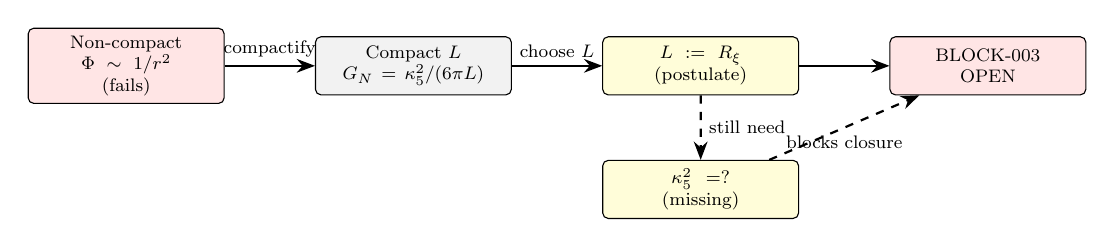
\begin{tikzpicture}[>=Stealth, node distance=1.4cm, scale=0.82, transform shape,
    box/.style={rectangle, draw, fill=gray!10, text width=2.8cm, text centered,
                minimum height=0.9cm, font=\footnotesize, rounded corners=2pt},
    failbox/.style={rectangle, draw, fill=red!10, text width=2.8cm, text centered,
                minimum height=0.9cm, font=\footnotesize, rounded corners=2pt},
    openbox/.style={rectangle, draw, fill=yellow!15, text width=2.8cm, text centered,
                minimum height=0.9cm, font=\footnotesize, rounded corners=2pt}]

    \node[failbox] (noncompact) {Non-compact\\$\Phi \sim 1/r^2$\\(fails)};
    \node[box, right=of noncompact] (compact) {Compact $L$\\$G_N = \kappa_5^2/(6\pi L)$};
    \node[openbox, right=of compact] (Lrxi) {$L := R_\xi$\\(postulate)};
    \node[openbox, below=1cm of Lrxi] (kappa) {$\kappa_5^2 = ?$\\(missing)};
    \node[failbox, right=of Lrxi] (outcome) {BLOCK-003\\OPEN};

    \draw[->, thick] (noncompact) -- (compact) node[midway, above, font=\footnotesize] {compactify};
    \draw[->, thick] (compact) -- (Lrxi) node[midway, above, font=\footnotesize] {choose $L$};
    \draw[->, thick, dashed] (Lrxi) -- (kappa) node[midway, right, font=\footnotesize] {still need};
    \draw[->, thick] (Lrxi) -- (outcome);
    \draw[->, thick, dashed] (kappa) -- (outcome) node[midway, below, font=\footnotesize] {blocks closure};
\end{tikzpicture}
\caption{Derivation attempt schematic (program overview; not to scale; not a result). Setting $L = R_\xi$ is consistent but does not close BLOCK-003 without an independent source for $\kappa_5^2$.}
\label{fig:schematic}
\end{figure}

%===============================================================================
\section{Outcome}
\label{sec:outcome}
%===============================================================================

\begin{failbox}
\textbf{Outcome: INCONCLUSIVE.}

\textbf{Attempt A} ($L = R_\xi$):
\begin{itemize}[nosep]
    \item Dimensionally consistent.
    \item Produces $G_N = \kappa_5^2 / (6\pi R_\xi)$.
    \item Does \emph{not} close BLOCK-003 because $\kappa_5^2$ is unspecified.
\end{itemize}

\textbf{Attempt B} ($L = \delta$):
\begin{itemize}[nosep]
    \item Two unknowns ($\kappa_5^2$, $\delta$); worse than Attempt A.
\end{itemize}

\textbf{Missing link:}
An EDC-internal derivation of $\kappa_5^2$ in terms of $(\sigma, R_\xi, \ldots)$.

\textbf{Thus BLOCK-003 remains OPEN.}
The derivation is narrowed to: ``Provide $\kappa_5^2 = f(\sigma, \ldots)$ from EDC geometry.''
\end{failbox}

%===============================================================================
\section{Conclusion}
\label{sec:conclusion}
%===============================================================================

\begin{enumerate}[nosep]
    \item Setting $L = R_\xi$ (weak-scale length) is a reasonable postulate for EDC compactification.
    \item This yields $G_N = \kappa_5^2 / (6\pi R_\xi)$, which is dimensionally correct.
    \item However, without $\kappa_5^2$ from EDC-internal physics, no prediction is made.
    \item The warped (RS-type) alternative offers $G_N \sim \kappa_5^4 \sigma$, but requires specifying $A(\xi)$.
    \item \textbf{BLOCK-003 remains OPEN}. The missing element is $\kappa_5^2 = f(\sigma, R_\xi, \ldots)$.
\end{enumerate}

\paragraph{Next step (out of scope for this note).}
Investigate whether EDC brane geometry or topological constraints can fix $\kappa_5^2$.
This would require analyzing the 5D bulk dynamics and their coupling to the brane tension.

\end{document}
